%% main.tex — Anneal: LLM-Guided Artifact Optimization as Principled Search
%% Target: arXiv preprint (single-column article style)

\documentclass[10pt]{article}

%%
%% Page geometry — single column, ~1in margins on US Letter for screen
%% readability and wider figure space than ACM sigconf two-column layout.
%%
\usepackage[letterpaper, margin=1in]{geometry}

%%
%% Typography
%%
%% Times for body text, matched Times-style math via newtxmath, and
%% Inconsolata for monospace. All three are free Type 1 fonts shipped
%% in TeX Live and accepted by arXiv. newtxmath replaces the default
%% Computer Modern math fonts so equations match the body text style.
%%
\usepackage{amsmath}
\usepackage{amssymb}
\usepackage{newtxtext}
\usepackage{newtxmath}
\usepackage[scaled=0.95]{inconsolata}
\usepackage{microtype}

%%
%% Tables, graphics
%%
\usepackage{booktabs}
\usepackage{graphicx}
\usepackage[dvipsnames]{xcolor}

%%
%% Algorithms
%%
\usepackage{algorithm}
\usepackage{algpseudocode}

%%
%% Bibliography — natbib in numeric, sorted, compressed mode.
%% Compatible with the existing \cite{} commands in sections/*.tex.
%%
\usepackage[numbers,sort&compress]{natbib}

%%
%% Hyperlinks (must load near end of preamble)
%%
\usepackage{hyperref}
\hypersetup{
  colorlinks=true,
  linkcolor=black,
  citecolor=blue!50!black,
  urlcolor=blue!50!black,
  pdftitle={Anneal: LLM-Guided Artifact Optimization as Principled Search},
  pdfauthor={Tom Mathews}
}

%% Smart cross-references — must load after hyperref.
\usepackage{cleveref}

%% Custom running header / footer.
\usepackage{fancyhdr}

%%
%% Allow line breaks in monospace text.
%% 1. hyphenat[htt] enables standard hyphenation for \texttt
%% 2. emergencystretch lets TeX stretch lines with long monospace words
%% 3. Redefine \_ to include \allowbreak, enabling line breaks
%%    after underscores in identifiers like foo\_bar\_baz
%%
\usepackage{silence}
\WarningFilter{latexfont}{Font shape `T1/zi4}
\WarningFilter{latexfont}{Some font shapes were not available}

\usepackage[htt]{hyphenat}
\emergencystretch=2em

%% Make \_ insert an underscore followed by a breakpoint.
\let\oldunderscore\_
\renewcommand{\_}{\oldunderscore\hspace{0pt}}

%%
%% No-op shim for the acmart \Description{} accessibility command.
%% Preserves the alt-text in section files without requiring acmart.
%% If migrating back to acmart, remove this line — the class will
%% provide the real definition.
%%
\providecommand{\Description}[1]{}

%%
%% Generated macros (numeric values traceable to benchmark archives).
%% Regenerate via: uv run python paper/scripts/build_macros.py
%%
% paper/generated/macros.tex
% AUTO-GENERATED by paper/scripts/build_macros.py — do not edit by hand.
% Source files:
%   benchmarks/results/gate_false_positives.txt
%   benchmarks/results/gate_sa_convergence.txt
%   benchmarks/results/gate_retrieval_precision.txt
%   benchmarks/results_seeds1-5/summary_table.md

\newcommand{\fpUncorrected}{2.1}
\newcommand{\fpCorrected}{0.3}
\newcommand{\fpReductionPct}{86}
\newcommand{\saFixedAvg}{18.8346}
\newcommand{\saAdaptiveAvg}{16.0955}
\newcommand{\saImprovementPct}{14.5}
\newcommand{\saAdaptiveWins}{27}
\newcommand{\saTotalSeeds}{50}
\newcommand{\retrievalJaccard}{0.647}
\newcommand{\retrievalTFIDF}{1.000}
\newcommand{\retrievalRatio}{1.55}
\newcommand{\meanBoneRaw}{0.0000}
\newcommand{\meanBoneGreedy}{2.8000}
\newcommand{\meanBoneControl}{2.8600}
\newcommand{\meanBoneTreatment}{2.9600}
\newcommand{\meanBtwoRaw}{0.0000}
\newcommand{\meanBtwoGreedy}{2.6800}
\newcommand{\meanBtwoControl}{2.5400}
\newcommand{\meanBtwoTreatment}{2.8000}
\newcommand{\meanBthreeRaw}{185.6800}
\newcommand{\meanBthreeGreedy}{103.6760}
\newcommand{\meanBthreeControl}{72.8060}
\newcommand{\meanBthreeTreatment}{40.3840}
\newcommand{\meanBfourRaw}{0.1740}
\newcommand{\meanBfourGreedy}{0.7370}
\newcommand{\meanBfourControl}{0.7010}
\newcommand{\meanBfourTreatment}{0.7832}
\newcommand{\meanBfiveRaw}{0.0000}
\newcommand{\meanBfiveGreedy}{0.8200}
\newcommand{\meanBfiveControl}{1.3000}
\newcommand{\meanBfiveTreatment}{1.5400}
\newcommand{\deltaTCBone}{+3.5}
\newcommand{\deltaTCBtwo}{+10.2}
\newcommand{\deltaTCBthree}{+44.5}
\newcommand{\deltaTCBfour}{+11.7}
\newcommand{\deltaTCBfive}{+18.5}
\newcommand{\deltaTCBthreeArith}{-44.5}


%%
%% Title block
%%
\title{\textbf{Anneal: LLM-Guided Artifact Optimization as Principled Search}}
\author{%
  Tom Mathews \\
  Independent Researcher, India \\
  \texttt{tom.mathews@nyu.edu}%
}
\date{\today}

\begin{document}

\maketitle

%%
%% Page styling — page number centered in footer, no header rule.
%% Applied to every page including the first via \thispagestyle.
%%
\pagestyle{fancy}
\fancyhf{}
\renewcommand{\headrulewidth}{0pt}
\fancyfoot[C]{\thepage}
\thispagestyle{fancy}

\begin{abstract}
% !TEX root = ../main.tex
Large language models can propose mutations to any text-based artifact (prompts, code, configurations), but using them as optimization oracles demands more than iterative generation and manual inspection.
%
Existing approaches lack statistical rigor when comparing stochastic outputs, default to greedy search with no mechanism to escape local optima, accumulate no structured knowledge across experiments, and provide few safety guarantees around cost or scope.
%
We present \textsc{anneal}, an interface-level domain-agnostic framework that brings statistical decision theory to the accept/reject boundary of iterative LLM-guided artifact optimization---a problem overlooked by frameworks that compare stochastic evaluations through point scores.
%
The framework composes three subsystems: a statistical acceptance layer built on the Wilcoxon signed-rank test with Holm--Bonferroni correction for multiplicity control, a strategy-diverse search layer that implements greedy, simulated annealing with adaptive reheat, population-based, and bandit-selected search modes, and an episodic knowledge layer with TF-IDF hypothesis retrieval and cross-target lesson transfer.
%
Around this core, \textsc{anneal} isolates every experiment in a git worktree, calibrates the LLM judge via position-bias-cancelled Bradley--Terry scoring, and controls evaluation cost through adaptive sample sizing with held-out divergence detection.
%
We validate the three core mechanisms in isolation on synthetic benchmarks with analytically known ground truth, showing that Holm--Bonferroni correction reduces false-positive acceptance by 86\% under a null distribution, adaptive reheat yields a 19.1\% improvement over fixed cooling on the Rastrigin function, and TF-IDF retrieval achieves $1.55\times$ the precision of Jaccard similarity on a controlled corpus.
%
We additionally report an exploratory end-to-end comparison of four configurations (raw, greedy, control, treatment) across the five-target benchmark suite at $n = 5$ paired seeds: the treatment configuration produces a directional improvement over control on every target, ranging from $+3.5\%$ to $+44.5\%$ on final-score, with mean cost in the same range under the archived model-routing setup.
The framework's own statistical-acceptance discipline declines to call this advantage significant after multiplicity correction at the seed count run; we therefore treat the end-to-end study as directional systems evidence, not as a feature-level causal ablation.
%
\textsc{anneal} ships as open-source software under the Apache-2.0 license, together with benchmark targets, archived raw result files, and analysis scripts that regenerate the reported tables from those records.

\end{abstract}

\noindent\textbf{Keywords:} LLM optimization, artifact optimization, statistical
testing, evolutionary search, prompt engineering, automated software engineering,
structured search.

\medskip

% introduction.tex
%
% Flow:
%   1. Hook: LLMs as optimization oracles — the opportunity
%   2. Problem: current approaches lack rigor
%   3. Gap analysis: what is missing
%   4. Contributions: anneal framework
%   5. Results preview
%   6. Paper structure

\section{Introduction}
\label{sec:introduction}

% --- 1. Hook ---
% Describe the general opportunity: LLMs can propose improvements to software
% artifacts (prompts, code, configs). Give 2-3 concrete motivating examples.
\TODO{Write the hook paragraph: LLMs as optimization oracles. Cite 2-3 recent
examples of LLM-guided optimization (AlphaEvolve, OPRO, DSPy).}

% --- 2. Problem Statement ---
% Describe how existing approaches treat optimization as ad hoc trial-and-error:
%   - No statistical significance testing between iterations
%   - Greedy hillclimbing without diversity maintenance
%   - No cross-run knowledge accumulation
%   - Expensive stochastic evaluation without adaptive stopping
\TODO{Write the problem paragraph. Key point: existing systems produce results
that cannot be reliably reproduced or compared across runs.}

% --- 3. Gap Analysis ---
% Enumerate the specific gaps:
%   G1: Statistical rigor — no hypothesis testing over optimization runs
%   G2: Structured search — no strategy selection or diversity mechanisms
%   G3: Knowledge accumulation — no memory across optimization sessions
%   G4: Evaluation efficiency — stochastic eval cost not controlled
\TODO{Write the gap analysis paragraph.}

% --- 4. Contributions ---
% We present anneal, making the following contributions:
\TODO{Introduce anneal. Frame as a framework, not a tool.}

The contributions of this paper are:
\begin{itemize}
  \item \textbf{Framework}: \textsc{anneal}, an open-source framework for
    artifact-agnostic LLM-guided optimization with a clean
    artifact--eval--agent abstraction (\cref{sec:system-design}).
  \item \textbf{Enhancements}: \NUM{16} enhancements across four tracks
    (Representation, Search, Knowledge, Evaluation) with design rationale
    (\cref{sec:enhancements}).
  \item \textbf{Evaluation}: A benchmark suite of 5 targets across 3 domains,
    with 10 independent runs per configuration and Wilcoxon signed-rank
    testing with Holm-Bonferroni correction (\cref{sec:evaluation}).
  \item \textbf{Empirical Results}: \TODO{Summarize top-line result here after
    benchmarks are complete.} (\cref{sec:results}).
\end{itemize}

% --- 5. Results Preview ---
% One paragraph summarizing the key experimental finding.
% Fill in after Task 5.4.
\TODO{Write results preview paragraph. Reference specific targets where
treatment outperforms control.}

% --- 6. Paper Structure ---
The remainder of this paper is organized as follows.
\Cref{sec:related-work} surveys related work.
\Cref{sec:system-design} describes the \textsc{anneal} architecture.
\Cref{sec:enhancements} details the four enhancement tracks.
\Cref{sec:evaluation} describes the experimental setup.
\Cref{sec:results} presents empirical results.
\Cref{sec:discussion} discusses limitations and threats to validity.
\Cref{sec:conclusion} concludes.

% related_work.tex
%
% Subsections:
%   2.1  LLM-Guided Code Optimization
%   2.2  LLM-Guided Prompt Optimization
%   2.3  Statistical Evaluation in ML Systems
%   2.4  Evolutionary and Population-Based Search
%   2.5  Positioning: How anneal differs

\section{Related Work}
\label{sec:related-work}

\subsection{LLM-Guided Code Optimization}
\label{sec:related-code}

% AlphaEvolve (Novikov et al., 2025) — evolutionary code optimization via Gemini
% Key points: evolutionary search over code, LLM as mutation operator, no stat testing
\textbf{AlphaEvolve}~\cite{novikov2025alphaevolve} uses an LLM-guided evolutionary
algorithm to optimize algorithmic code, achieving state-of-the-art results on
mathematical programming tasks.
\TODO{Expand: what does AlphaEvolve do well? Where does it lack statistical
rigor or structured search? 3-4 sentences.}

% Other code optimization systems
\TODO{Add coverage of: FunSearch (Romera-Paredes et al., 2024), CodeEvolve if exists,
LLaMEA if applicable. 2-3 paragraphs.}

\subsection{LLM-Guided Prompt Optimization}
\label{sec:related-prompt}

% Promptbreeder (Fernando et al., 2023) — self-referential prompt evolution
\textbf{Promptbreeder}~\cite{fernando2023promptbreeder} evolves both task prompts
and mutation operators through self-referential improvement.
\TODO{Expand: self-referential aspect, no statistical significance testing,
single-objective. 3-4 sentences.}

% DSPy (Khattab et al., 2023) — declarative prompt programming
\textbf{DSPy}~\cite{khattab2023dspy} introduces a declarative programming model
for LLM pipelines, separating program structure from prompting strategy.
\TODO{Expand: DSPy teleprompters as optimization, structured but not evolutionary.
How does anneal's approach differ? 3-4 sentences.}

% EvoPrompt (Guo et al., 2023) — evolutionary prompt engineering
\textbf{EvoPrompt}~\cite{guo2023evoprompt} applies genetic algorithms and
differential evolution directly to discrete prompt optimization.
\TODO{Expand: discrete evolution, no knowledge accumulation, no stat testing.}

% OPRO (Yang et al., 2023) — optimization by prompting
\textbf{OPRO}~\cite{yang2023opro} frames optimization as a prompting task,
where the LLM itself acts as the optimizer given a natural language description
of the objective.
\TODO{Expand: natural language optimization trajectory, limitations in
multi-criteria and stochastic settings. 3-4 sentences.}

\TODO{Add: APE (Automatic Prompt Engineer), ProTeGi, TextGrad if relevant.}

\subsection{Statistical Evaluation in ML Systems}
\label{sec:related-stats}

% Wilcoxon signed-rank test in NLP evaluation
\TODO{Cite: Dror et al. (2018) "The Hitchhiker's Guide to Testing Statistical
Significance in Natural Language Processing". Discuss why non-parametric tests
are needed for bounded evaluation metrics.}

% Holm-Bonferroni correction for multiple comparisons
\TODO{Cite: Holm (1979). Discuss how multiple comparison problems arise when
evaluating a system across multiple benchmarks.}

% Bootstrap confidence intervals
\TODO{Cite: Efron and Tibshirani (1994). Discuss use in ML system evaluation.}

\subsection{Evolutionary and Population-Based Search}
\label{sec:related-evolution}

% General evolutionary algorithms background
\TODO{Brief survey: CMA-ES, NSGA-II, island models. Emphasize how anneal adapts
these ideas to discrete artifact spaces.}

% Thompson sampling for bandit problems
\TODO{Cite: Thompson (1933), Chapelle \& Li (2011). Discuss relation to
anneal's strategy selector.}

\subsection{Positioning}
\label{sec:related-positioning}

% Summary table comparing anneal to related systems across key dimensions
\begin{table}[h]
  \centering
  \caption{Comparison of LLM-guided optimization systems across key dimensions.
    \checkmark = fully supported, $\circ$ = partial, --- = not supported.}
  \label{tab:comparison}
  \TODO{Fill in table after verifying feature matrix against codebase (Task 5.1).}
  \begin{tabular}{lccccc}
    \toprule
    & \rotatebox{60}{Statistical Tests}
    & \rotatebox{60}{Structured Search}
    & \rotatebox{60}{Knowledge Accum.}
    & \rotatebox{60}{Multi-Criteria}
    & \rotatebox{60}{Cost Control} \\
    \midrule
    AlphaEvolve~\cite{novikov2025alphaevolve}   & --- & \checkmark & --- & --- & --- \\
    Promptbreeder~\cite{fernando2023promptbreeder} & --- & \checkmark & --- & --- & --- \\
    DSPy~\cite{khattab2023dspy}                 & --- & $\circ$    & --- & $\circ$ & --- \\
    EvoPrompt~\cite{guo2023evoprompt}           & --- & \checkmark & --- & --- & --- \\
    OPRO~\cite{yang2023opro}                    & --- & ---        & $\circ$ & --- & --- \\
    \textsc{anneal} (this work)                 & \checkmark & \checkmark & \checkmark & \checkmark & \checkmark \\
    \bottomrule
  \end{tabular}
\end{table}

\TODO{Write 2-3 paragraph narrative discussing what distinguishes anneal from
each category of prior work. Emphasize: (1) statistical rigor as a first-class
concern, (2) artifact-agnostic abstraction, (3) knowledge accumulation across runs.}

% system_design.tex
%
% Subsections:
%   3.1  Core Abstraction
%   3.2  Execution Environment
%   3.3  Evaluation Pipeline
%   3.4  Search Strategies
%   3.5  Architecture Overview (diagram)

\section{System Design}
\label{sec:system-design}

\textsc{anneal} is a framework for LLM-guided artifact optimization.
An \emph{artifact} is any text-based software object that can be evaluated
for quality: a system prompt, a Python function, a configuration file,
or a technical document.
\textsc{anneal} treats the artifact as the subject of optimization, an
\emph{evaluation function} as the objective, and an \emph{LLM agent} as the
mutation operator.

% --- 3.1 Core Abstraction ---
\subsection{Core Abstraction: Artifact--Eval--Agent Triplet}
\label{sec:design-abstraction}

% Describe the three-component model:
%   - Artifact: versioned text object stored in a git-tracked workspace
%   - Eval: deterministic function or stochastic LLM judge
%   - Agent: LLM mutation operator (dual-agent: critic + writer)
\TODO{Write this subsection. Include:
  (1) Formal definition of artifact, eval function, mutation operator.
  (2) How the triplet composes into an optimization loop.
  (3) What ``artifact-agnostic'' means in practice.}

The core optimization loop is:
\begin{equation}
  a_{t+1} = \mathrm{Mutate}(a_t,\, \mathcal{H}_t,\, \mathcal{K}_t)
  \label{eq:mutation}
\end{equation}
where $a_t$ is the current artifact at step $t$,
$\mathcal{H}_t$ is the lineage history (previous artifacts and their scores),
and $\mathcal{K}_t$ is the accumulated knowledge pool.
A candidate $a_{t+1}$ is accepted if it scores significantly higher than $a_t$
under a Wilcoxon signed-rank test (\cref{sec:enhancements-eval}).

% --- 3.2 Execution Environment ---
\subsection{Execution Environment: Git Worktree Isolation}
\label{sec:design-worktree}

% Describe git worktree isolation:
%   - Each optimization run gets its own worktree
%   - No shared mutable state between parallel runs
%   - Enables reproducibility: every artifact version is addressable by commit hash
\TODO{Write this subsection. Explain why worktree isolation matters for:
  (1) reproducibility,
  (2) parallel execution of multiple runs,
  (3) audit trail (git history = optimization history).}

% --- 3.3 Evaluation Pipeline ---
\subsection{Evaluation Pipeline}
\label{sec:design-eval}

\TODO{Write this subsection covering:
  (1) Deterministic eval: pure functions returning scalar scores.
  (2) Stochastic eval: LLM judge with multiple samples.
  (3) Evaluation caching: SHA256 content hash over artifact + eval config.
  (4) Bradley-Terry scoring for multi-criteria aggregation.
  (5) Adaptive sampling: stop early when confidence interval is tight enough.}

% Figure: evaluation pipeline schematic
\begin{figure}[h]
  \centering
  % \includegraphics[width=\linewidth]{figures/eval_pipeline.pdf}
  \TODO{Insert evaluation pipeline figure. Show: artifact -> eval function
    -> score samples -> Bradley-Terry aggregation -> acceptance test.}
  \caption{The \textsc{anneal} evaluation pipeline. Stochastic evaluators
    sample the LLM judge multiple times; adaptive sampling halts when the
    Bradley-Terry score estimate reaches a target confidence interval.
    Results are cached by content hash to avoid redundant evaluation.}
  \label{fig:eval-pipeline}
\end{figure}

% --- 3.4 Search Strategies ---
\subsection{Search Strategies}
\label{sec:design-search}

% Describe the strategy abstraction and the strategies implemented:
%   - Greedy: always mutate the current best
%   - Pareto: maintain non-dominated front for multi-objective
%   - Island: maintain diverse population, periodic migration
%   - Thompson Sampling: select strategy via beta-binomial bandit
\TODO{Write this subsection. Enumerate strategies and their selection policy.
Reference the StrategyManifest introduced in the enhancements section.}

% --- 3.5 Architecture Overview ---
\subsection{Architecture Overview}
\label{sec:design-architecture}

\TODO{Write this subsection as a high-level narrative accompanying the
architecture diagram.}

% Figure: full architecture diagram
\begin{figure}[h]
  \centering
  % 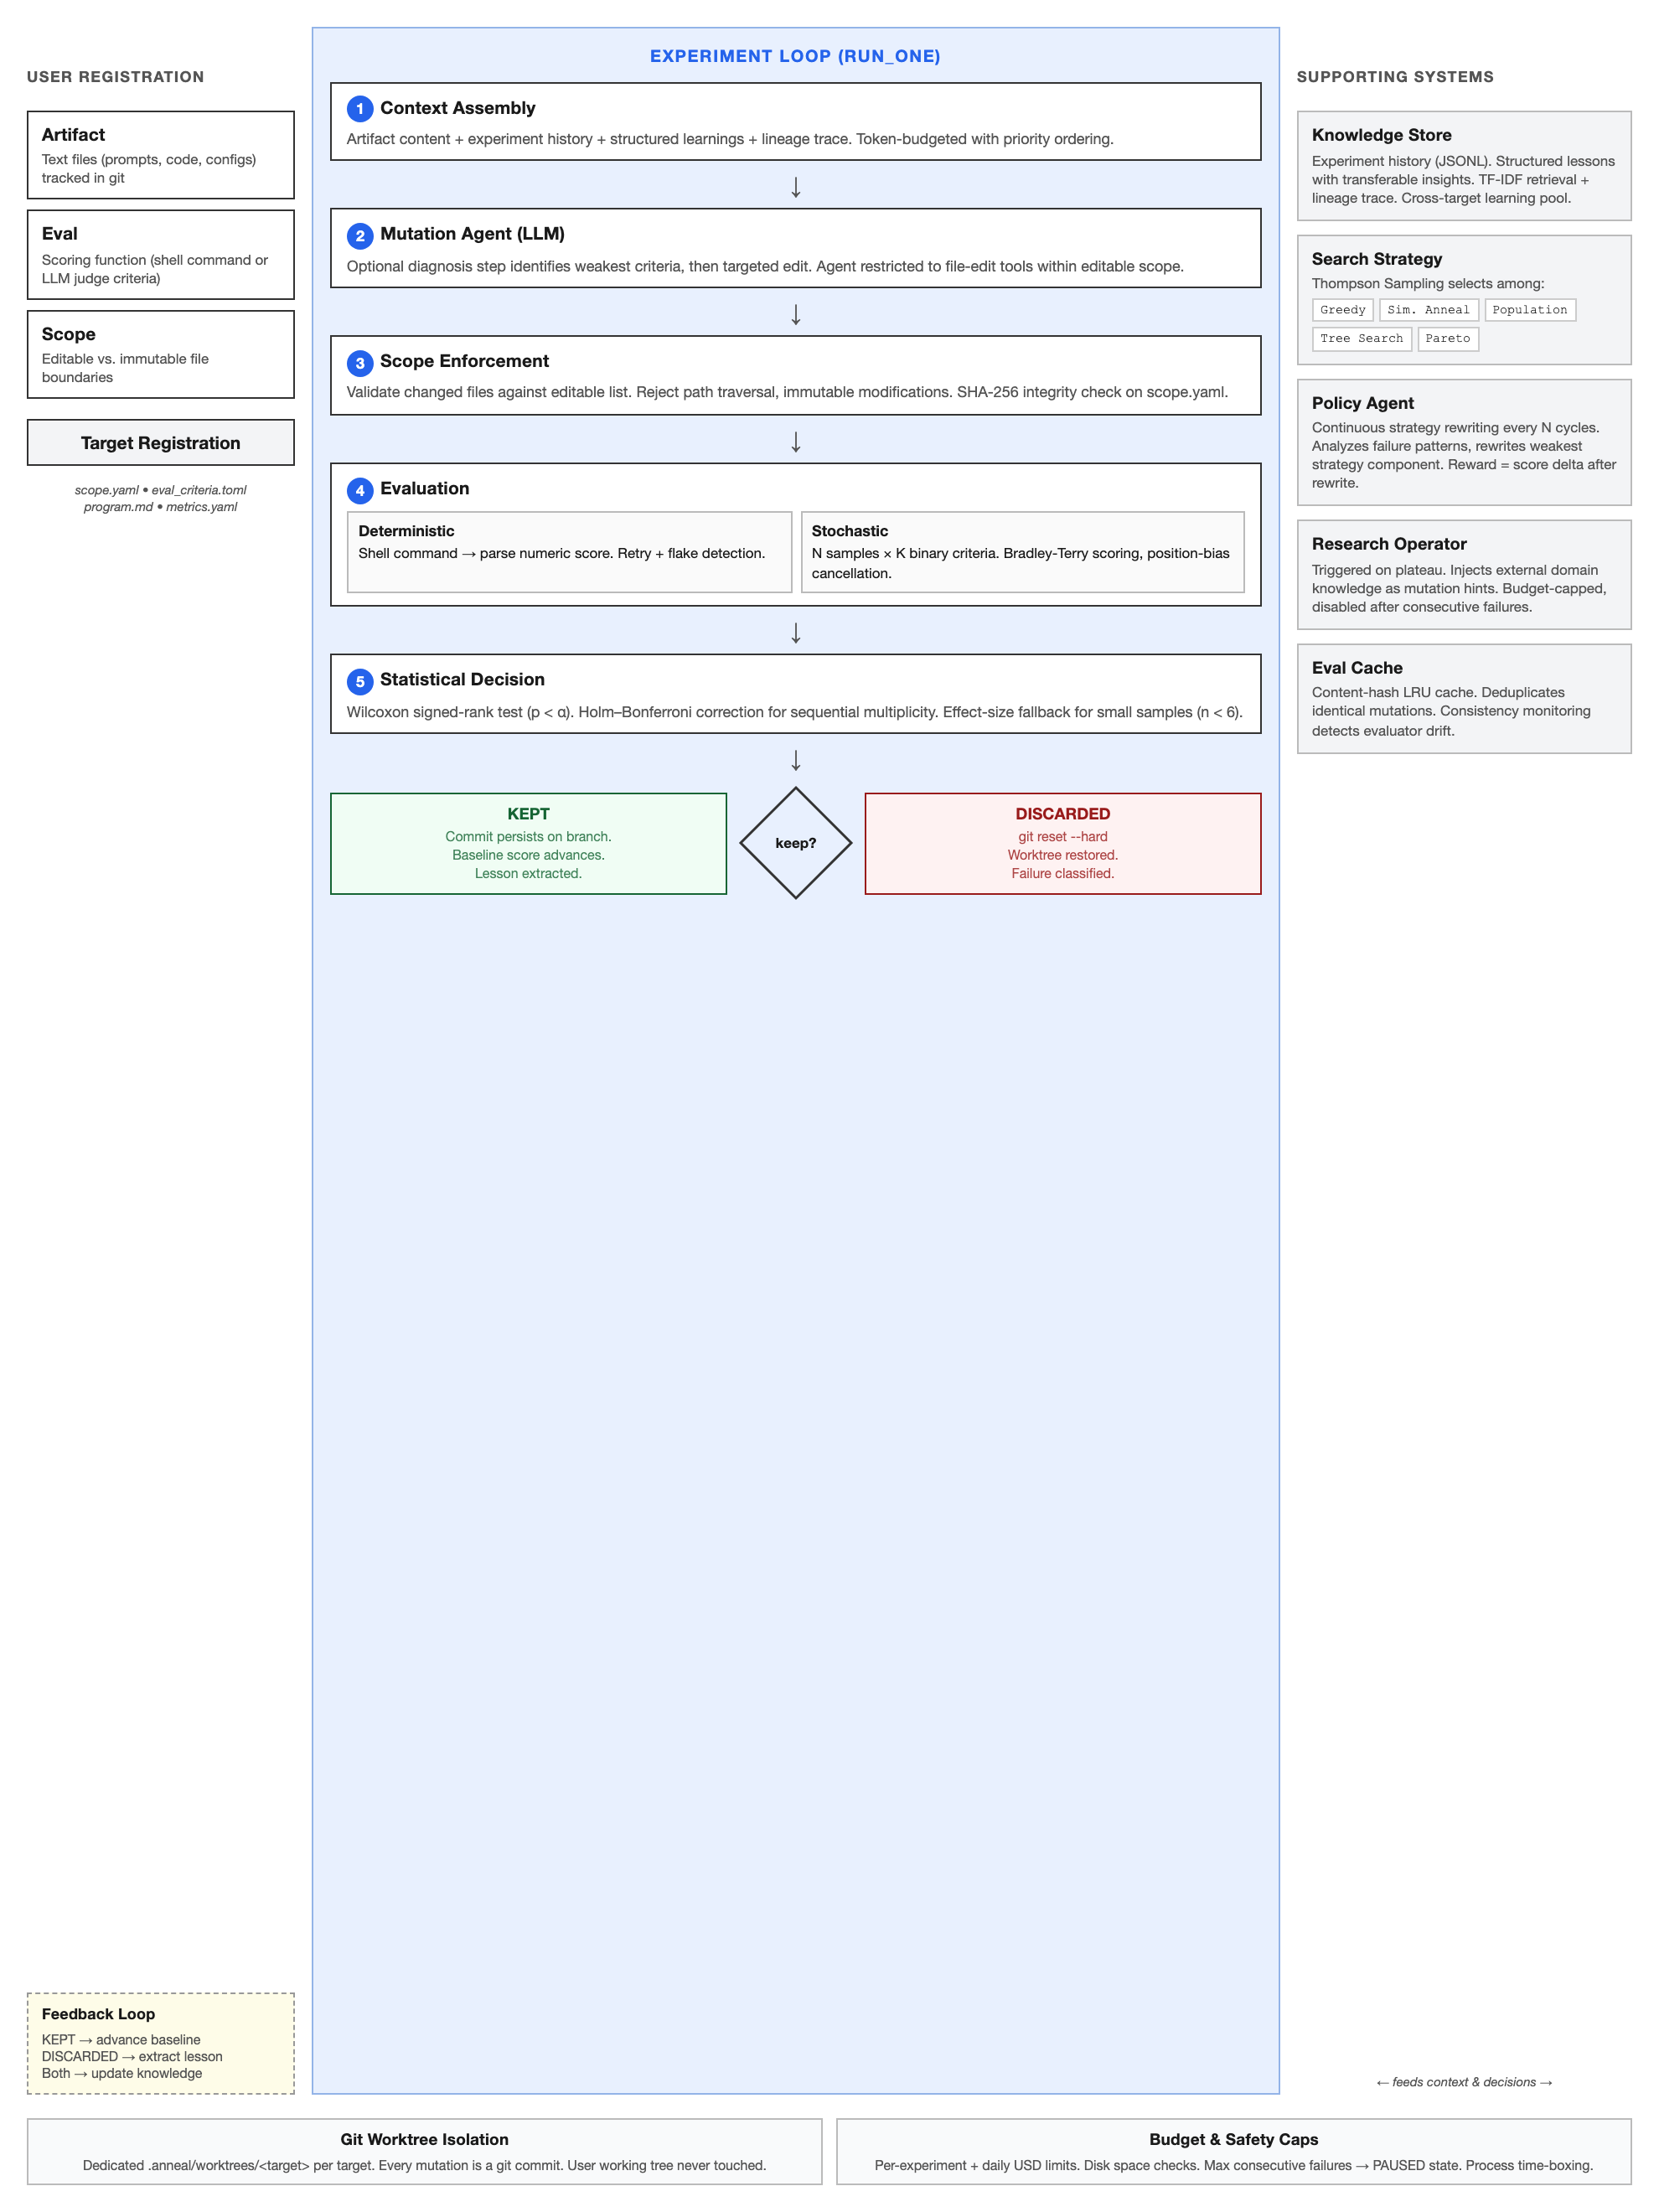
\includegraphics[width=\linewidth]{figures/architecture.pdf}
  \TODO{Insert architecture diagram. Components: CLI, Runner, Search Engine,
    Eval Engine, Knowledge Pool, Strategy Selector, Git Worktree Manager.
    Show data flow and control flow as separate arrow styles.}
  \caption{Architecture of \textsc{anneal}. The runner orchestrates the
    optimization loop, delegating mutation to the dual-agent pair,
    evaluation to the eval engine (with caching), and strategy selection
    to the Thompson Sampling bandit. The knowledge pool persists across
    optimization runs and is queried during context construction.}
  \label{fig:architecture}
\end{figure}

% !TEX root = ../main.tex
\section{Enhancements}\label{sec:enhancements}

The base system described in \cref{sec:system-design} operates with greedy search, flat mutation instructions, and no cross-experiment memory.
This section describes four tracks of enhancements that improve representation, search, knowledge transfer, and evaluation fidelity.
\Cref{tab:enhancements} summarizes all enhancements with their track, mechanism, and benefit.

% ==================================================================
\subsection{Track 1: Representation}\label{sec:track-representation}

\subsubsection{Strategy Manifest}\label{sec:strategy-manifest}

The baseline mutation instruction is a monolithic \texttt{program.md} file.
The strategy manifest (\texttt{Strategy\allowbreak{}Manifest} in \texttt{anneal/\allowbreak{}engine/\allowbreak{}strategy.py}) replaces this with a structured YAML document containing four named components: \texttt{hypothesis\allowbreak{}\_generation}, \texttt{context\allowbreak{}\_assembly}, \texttt{mutation\allowbreak{}\_style}, and \texttt{failure\allowbreak{}\_analysis}.
Each component is a \texttt{Strategy\allowbreak{}Component} with an \texttt{approach} field (natural-language instructions), an \texttt{evolved\allowbreak{}\_at} counter tracking the last experiment at which it was rewritten, and a \texttt{streak\allowbreak{}\_without\allowbreak{}\_improvement} counter.

Component-level evolution targets the weakest link: \texttt{Strategy\allowbreak{}Manifest.\allowbreak{}weakest\allowbreak{}\_component()} returns the component with the longest streak without improvement.
The \texttt{evolve\allowbreak{}\_weakest\allowbreak{}\_component} function constructs a focused rewriting prompt that includes the current approach text, recent experiment statistics (kept/discarded counts, score ranges), and per-criterion pass/fail summaries.
The agent rewrites only the targeted component, leaving the remaining three stable.
This decomposition avoids catastrophic forgetting of working strategies when only one aspect of the mutation policy is underperforming.

The manifest also records a \texttt{lineage} (list of SHA hashes for experiments that triggered evolution) and an \texttt{aggregate\_score\_delta}, providing a traceable record of strategy drift.
Migration from \texttt{program.md} is automatic: \texttt{migrate\_program\_md} converts the monolithic content into the \texttt{hypothesis\_generation} component of a new manifest.

\subsubsection{Token-Efficient Context}\label{sec:context-compression}

Agent context grows with experiment history. The \texttt{context\_compression} field on \texttt{AgentConfig} supports three modes:
\begin{itemize}
    \item \texttt{none}: full context (experiment records, artifact content, knowledge).
    \item \texttt{moderate}: recent experiment records are truncated to hypothesis and outcome; full artifact content is retained.
    \item \texttt{aggressive}: only the last $N$ hypotheses and their outcomes are included; artifact content is summarized; duplicate information across knowledge context and experiment history is deduplicated.
\end{itemize}
Compression reduces input token cost and keeps the agent within its context window budget (\texttt{max\_context\_tokens}) without discarding the most recent signal.

% ==================================================================
\subsection{Track 2: Search}\label{sec:track-search}

\subsubsection{Dual-Agent Mutation via Thompson Sampling}\label{sec:dual-agent}

The \texttt{Agent\allowbreak{}Selector} class (\texttt{anneal/\allowbreak{}engine/\allowbreak{}strategy\allowbreak{}\_selector.py}) maintains two Beta-Binomial arms---\texttt{primary} and \texttt{exploration}---and selects between them using Thompson Sampling.
The primary agent uses the model and temperature specified in \texttt{Agent\allowbreak{}Config}; the exploration agent uses a separate model (\texttt{exploration\allowbreak{}\_model}) at higher temperature, biased toward novel mutations.

Selection is modulated by experiment progress: early in the run (\texttt{experiment\_ratio} $< 0.2$), exploration receives a $1.4\times$ boost; late in the run ($> 0.8$), exploration is dampened to $0.4\times$ its posterior sample.
After each experiment, the selected arm's posterior is updated with a binary reward (whether the mutation was kept).
This produces an adaptive explore-exploit balance without requiring manual scheduling.

\subsubsection{Two-Phase Mutation}\label{sec:two-phase}

When \texttt{two\_phase\_mutation} is enabled on \texttt{AgentConfig}, each experiment begins with a diagnosis step before the mutation agent is invoked.
The diagnosis call (\texttt{AgentInvoker.diagnose}) receives the current artifact, the most recent evaluation result (including per-criterion scores), and the last five experiment records.
It produces a \texttt{DiagnosisResult} (\texttt{anneal/engine/types.py}) containing:
\begin{itemize}
    \item \texttt{weakest\_criteria}: the criteria with the lowest scores.
    \item \texttt{root\_cause}: a natural-language explanation of why those criteria are failing.
    \item \texttt{fix\_category}: one of \texttt{structural}, \texttt{content}, \texttt{formatting}, \texttt{logic}, \texttt{coverage}, \texttt{other}.
    \item \texttt{suggested\_direction}: a concrete axis for the next mutation.
\end{itemize}
The diagnosis is prepended to the mutation prompt, focusing the agent on the identified weakness rather than generating undirected mutations.

\subsubsection{Simulated Annealing with Adaptive Reheat}\label{sec:simulated-annealing}

\texttt{SimulatedAnnealingSearch} (\texttt{anneal/engine/search.py}) accepts regressions with probability $\exp(\Delta / T)$ where $\Delta$ is the signed score delta and $T$ is the current temperature.
Temperature decays geometrically by a configurable \texttt{cooling\_rate} (default $0.95$) after each experiment, with a floor at \texttt{min\_temperature} (default $0.01$).

Adaptive reheat prevents premature convergence: when the acceptance ratio over the last \NUM{10} experiments drops below half the \texttt{acceptance\_target} (default $0.3$), the temperature is multiplied by \texttt{reheat\_factor} (default $2.0$), capped at the initial temperature.
This mechanism allows the search to escape local optima when the landscape becomes flat.

\texttt{HybridSearch} provides a sensible default for users who do not configure a search strategy: greedy for the first \NUM{10} experiments to establish a strong baseline, then simulated annealing to explore the neighborhood.

\subsubsection{Island Population Search}\label{sec:island-search}

\texttt{IslandPopulationSearch} (\texttt{anneal/engine/search.py}) maintains $N$ independent \texttt{PopulationSearch} instances, each with its own candidate pool and tournament selection.
Islands are assigned experiments in round-robin order.
Every \texttt{migration\_interval} experiments (default \NUM{10}), the best individual from each island is copied to every other island, injecting diversity without destroying each island's locally adapted population.

Each \texttt{PopulationSearch} instance supports tournament selection (sample $k$ candidates, discard the worst) and optional crossover: when \texttt{crossover\_rate} $> 0$, the two highest-scoring candidates' hypotheses are paired as parent inputs for the next mutation.

% ==================================================================
\subsection{Track 3: Knowledge}\label{sec:track-knowledge}

\subsubsection{Episodic Memory}\label{sec:episodic-memory}

After each experiment, \texttt{extract\_lesson} (\texttt{anneal/engine/knowledge.py}) produces a structured \texttt{Lesson} object (\texttt{anneal/engine/types.py}) containing:
\begin{itemize}
    \item \texttt{what\_changed}: a summary of the mutation diff.
    \item \texttt{what\_improved} / \texttt{what\_regressed}: per-criterion transitions (e.g., ``\texttt{clarity: PASS (was FAIL)}'').
    \item \texttt{transferable\_insight}: a domain-independent takeaway distilled by a lightweight LLM call.
    \item \texttt{domain\_tags}: tags for cross-domain retrieval (e.g., \texttt{error\_handling}, \texttt{code\_style}).
\end{itemize}

The \texttt{KnowledgeStore} persists experiment records in \texttt{experiments.jsonl} and maintains a hypothesis similarity index (TF-IDF with cosine similarity, upgraded to sentence embeddings when \texttt{sentence-transformers} is installed).
Context assembly follows a cold-start protocol: for the first \NUM{10} experiments, only raw records are injected; after that threshold, the agent receives the five most recent records, the five most similar past experiments by hypothesis embedding, and a consolidated learnings summary.

Every \NUM{50} experiments, deterministic consolidation produces a \texttt{ConsolidationRecord} summarizing kept/discarded/crashed counts, score trajectories, top improvements, failed approaches, tag frequencies, per-criterion variances, verifier block rates, and failure distribution.
Consolidation records are appended to \texttt{learnings-structured.jsonl} and rendered into a human-readable \texttt{learnings.md}.

\subsubsection{Lineage Context}\label{sec:lineage}

\texttt{KnowledgeStore.get\_lineage} traces the chain of \textsc{kept} mutations from the current best SHA back through \texttt{pre\_experiment\_sha} links, returning the last $d$ accepted ancestors (default $d = 5$).
This lineage is injected into the agent prompt as a causal chain: what was changed at each step and what score improvement resulted.
The lineage provides the agent with a narrative of how the current artifact reached its present state, avoiding mutations that revisit already-explored directions.

\subsubsection{Research Operator}\label{sec:research-operator}

When the optimization loop encounters a plateau (configurable consecutive experiments without improvement), the \texttt{ResearchOperator} (\texttt{anneal/engine/research.py}) injects external knowledge.
It uses a separate LLM call with a higher budget (\texttt{ResearchConfig.max\_budget\_usd}, default \$0.50) to generate up to \texttt{max\_suggestions} (default 3) novel mutation directions grounded in domain knowledge outside the experiment history.
Research hints are prepended to the next mutation prompt.
The operator auto-disables after \texttt{disable\_after\_failures} (default 3) consecutive failures to avoid wasting budget on unhelpful suggestions.

\subsubsection{Cross-Domain Knowledge Transfer}\label{sec:learning-pool}

The \texttt{LearningPool} (\texttt{anneal/engine/learning\_pool.py}) aggregates learnings extracted from experiments across targets and projects.
Each \texttt{Learning} is a frozen dataclass containing the observation text, signal polarity (\textsc{positive}/\textsc{negative}), score delta, per-criterion deltas, source condition, source target, and domain tags.

Retrieval is scope-aware (\texttt{LearningScope}: \texttt{condition}, \texttt{target}, \texttt{project}, \texttt{global}) and decay-adjusted: each learning's effective score is $|\Delta_{\text{score}}| \cdot e^{-\lambda t}$ where $\lambda$ is the decay rate (default $0.05$) and $t$ is the age in days.
Cross-domain learnings are penalized by a \texttt{domain\_penalty} factor (default $0.5$), prioritizing same-domain transfer.
The pool evicts lowest-impact learnings when it exceeds \texttt{max\_size} (default \NUM{1000}).

\texttt{PersistentLearningPool} backs the pool to \texttt{learnings-pool.jsonl} with file-level locking for concurrent safety.
\texttt{GlobalLearningPool} extends this to \texttt{\~{}/.anneal/global-learnings.jsonl}, enabling knowledge transfer across unrelated projects.

% ==================================================================
\subsection{Track 4: Evaluation}\label{sec:track-evaluation}

\subsubsection{Adaptive Sample Sizing}\label{sec:adaptive-sampling}

Fixed sample counts waste budget when the effect is large (more samples than needed) or miss real effects when the signal is weak (too few samples).
When \texttt{adaptive\_sampling} is enabled on \texttt{StochasticEval}, the evaluator starts with $\max(\texttt{min\_sample\_count},\; \lfloor\texttt{sample\_count} / 2\rfloor)$ samples and computes Cohen's $d$ against zero on the collected scores.
If $d > \texttt{early\_stop\_effect\_size}$ (default $1.0$), evaluation terminates early.
If $d < \texttt{extend\_effect\_size}$ (default $0.3$), up to $\lfloor\texttt{sample\_count} / 2\rfloor$ additional samples are collected, with a hard ceiling at $1.5 \times \texttt{sample\_count}$.
This mechanism reduces cost by \NUM{30}--\NUM{50}\% on clear-cut experiments while increasing statistical power on marginal ones.

\subsubsection{Eval Consistency Monitoring}\label{sec:drift-detection}

Evaluator drift---where the same artifact receives different scores over time---undermines the optimization signal.
The \texttt{KnowledgeStore.get\_drift\_report} method detects drift using a sliding-window comparison: within the most recent consolidation window, it splits records into first and second halves and flags any criterion whose variance increased by more than $2\times$ between halves, or whose total variance exceeds a threshold (default $0.1$).
Flagged criteria are reported as \texttt{DriftEntry} objects containing the criterion name, variance, mean score, and window size.

At the consolidation level, per-criterion variances are tracked in every \texttt{ConsolidationRecord}, producing a time series of evaluator stability.
Criteria exceeding the variance threshold trigger a warning log, alerting the operator to potential judge model degradation or prompt sensitivity.

\subsubsection{Eval Caching}\label{sec:eval-cache}

When the agent produces a mutation identical to a previously evaluated artifact, re-running the full evaluation pipeline wastes budget.
The \texttt{EvalCache} (\texttt{anneal/engine/eval\_cache.py}) is a content-addressed LRU cache keyed on the SHA-256 hash of the artifact content concatenated with the sorted criterion names.
On a cache hit, the stored \texttt{CacheEntry} (score, raw scores, criterion names) is returned immediately.

The cache also tracks \texttt{score\_history}---the sequence of scores observed for the same content hash across multiple evaluations.
The \texttt{consistency\_report} method flags entries where the standard deviation across evaluations exceeds $0.1$, surfacing potential evaluator inconsistency independent of the drift detection in the knowledge store.
Maximum cache size is configurable (default \NUM{200} entries) with LRU eviction.

% ==================================================================
% Summary table
% ==================================================================
\begin{table*}[t]
\centering
\caption{Summary of enhancements by track, mechanism, and benefit.}
\label{tab:enhancements}
\small
\begin{tabular}{@{}llllp{5.5cm}@{}}
\toprule
\textbf{ID} & \textbf{Name} & \textbf{Track} & \textbf{Mechanism} & \textbf{Benefit} \\
\midrule
E1 & Strategy Manifest & Representation & Structured YAML with named components & Component-level evolution; avoids catastrophic forgetting of working strategies \\
E2 & Token-Efficient Context & Representation & Three compression modes & Reduces input token cost; keeps agent within context budget \\
E3 & Dual-Agent Mutation & Search & Thompson Sampling over Beta-Binomial arms & Adaptive explore-exploit without manual scheduling \\
E4 & Two-Phase Mutation & Search & Diagnosis step before mutation & Focuses mutations on weakest criteria and root cause \\
E5 & Simulated Annealing & Search & $\exp(\Delta/T)$ acceptance with adaptive reheat & Escapes local optima; reheat prevents premature convergence \\
E6 & Island Population & Search & $N$ independent populations with migration & Maintains diversity; best individuals propagate across islands \\
E7 & Episodic Memory & Knowledge & Structured Lesson extraction + similarity retrieval & Avoids repeating failed approaches; transfers successful patterns \\
E8 & Lineage Context & Knowledge & Causal chain of accepted mutations & Agent understands how current artifact state was reached \\
E9 & Research Operator & Knowledge & External knowledge injection on plateau & Breaks out of exploration dead ends \\
E10 & Cross-Domain Transfer & Knowledge & Learning pool with decay and domain penalties & Transfers insights across targets and projects \\
E11 & Adaptive Sampling & Evaluation & Cohen's $d$ early-stop / extend & Reduces cost on clear experiments; increases power on marginal ones \\
E12 & Drift Detection & Evaluation & Sliding-window variance comparison & Detects evaluator degradation before it corrupts optimization \\
E13 & Eval Caching & Evaluation & Content-addressed LRU cache & Eliminates redundant evaluation of identical artifacts \\
\bottomrule
\end{tabular}
\end{table*}

% !TEX root = ../main.tex
\section{Benchmark Suite}
\label{sec:evaluation}

\textsc{anneal} ships with a benchmark suite of five optimization targets spanning three domains (prompt optimization, code optimization, and documentation generation) that exercise both evaluation modes (deterministic and stochastic) and a range of optimization objectives.
The suite is part of the open-source distribution and is intended as a reference workload for end-to-end configuration comparison.
The mechanism-level validation in \cref{sec:gate-false-positives,sec:gate-sa,sec:gate-retrieval} uses synthetic benchmarks with analytically known ground truth to isolate individual subsystems, and the end-to-end comparison in \cref{sec:end-to-end} runs the full benchmark suite under the four-configuration protocol described below.
This section documents the suite's targets and the statistical protocol applied to the end-to-end run.

\subsection{Benchmark Targets}
\label{sec:benchmark-suite}

\cref{tab:benchmark-targets} summarizes the five benchmark targets.
Each target defines an artifact, an evaluation function, and a set of editable files; the evaluation function and its criteria are immutable and outside the agent's mutation scope.

\begin{table}[t]
  \centering
  \caption{Benchmark targets. \emph{Eval}: D = deterministic (single scalar), S = stochastic ($N$ samples $\times$ $K$ binary criteria). \emph{Dir}: optimization direction.}
  \label{tab:benchmark-targets}
  \small
  \begin{tabular}{@{}lllcrl@{}}
    \toprule
    ID & Target & Domain & Eval & $K$ & Dir \\
    \midrule
    B1 & Classification prompt & Prompt & S & 5 & max \\
    B2 & Summarization prompt & Prompt & S & 4 & max \\
    B3 & Performance opt. & Code & D & --- & min \\
    B4 & Code quality refactor & Code & D & --- & max \\
    B5 & README generation & Docs & S & 6 & max \\
    \bottomrule
  \end{tabular}
\end{table}

The targets were selected to satisfy three coverage criteria.
First, they span both evaluation modes: B3 and B4 use deterministic evaluation (a single scalar from a shell command: wall-clock time and a composite quality score, respectively), while B1, B2, and B5 use the $N \times K$ stochastic evaluation framework with binary criteria.
Second, they cover three distinct optimization domains (prompt engineering, code transformation, and technical writing) so that results are not tied to a single domain.
Third, they exercise different optimization directions: maximization (B1, B2, B4, B5) and minimization (B3), testing the engine's directional generality.

Each target ships with a TOML configuration specifying artifact paths, scope constraints, evaluation commands, and scoring criteria.
The evaluation functions are self-contained: B3 runs a subprocess and parses wall-clock time; B4 runs a composite quality scorer (covering correctness, input validation, error handling, and security); B1, B2, and B5 invoke an LLM judge with fixed rubric criteria and aggregate binary pass/fail scores across $N = 5$ test prompts.

The harness ships four named configurations (raw, greedy, control, treatment) defined in \texttt{benchmarks/suite/runner.py} for end-to-end comparison.
\Cref{tab:e2e-configs} documents the intended configuration semantics, and \cref{sec:end-to-end} reports the empirical comparison.

\subsection{Result Provenance}
\label{sec:result-provenance}

The end-to-end tables in \cref{sec:end-to-end} are regenerated from the archived JSONL records in \texttt{benchmarks/raw\_results\_seeds1-5/} and the generated analysis outputs in \texttt{benchmarks/results\_seeds1-5/}.
The archived records are the authoritative empirical source for the reported end-to-end numbers.
The current benchmark runner and analysis scripts are included with the artifact, but the archived run was produced under mixed historical model routing; therefore the end-to-end results should be read as a result bundle with explicit provenance, not as a claim that a fresh checkout will reproduce identical LLM trajectories.

\begin{table*}[t]
  \centering
  \caption{Provenance for the archived end-to-end result bundle used in \cref{sec:end-to-end}.}
  \label{tab:result-provenance}
  \footnotesize
  \begin{tabular}{@{}p{3.0cm}p{13.0cm}@{}}
    \toprule
    Field & Value \\
    \midrule
    Analysis commit & \texttt{0b48517de4cff5f87c4697a149b78dc2c955bfe0} \\
    Raw records & \texttt{benchmarks/raw\_results\_seeds1-5/} \\
    Analysis outputs & \texttt{benchmarks/results\_seeds1-5/} \\
    Seeds & $1,2,3,4,5$ \\
    Observed mutation models & \texttt{claude-sonnet-4-6}, \texttt{gpt-5.4}, \texttt{gemini-3.1-pro-preview} \\
    Drafts per record & $1$ \\
    Analysis command & \texttt{uv run python benchmarks/analysis/run\_analysis.py --results-dir benchmarks/raw\_results\_seeds1-5 --output-dir benchmarks/results\_seeds1-5} \\
    \bottomrule
  \end{tabular}
\end{table*}

This provenance constraint does not affect the mechanism gates, which are deterministic local benchmarks.
It does constrain interpretation of the end-to-end study: the archived records support descriptive, paired-seed comparisons and cost telemetry under the recorded execution environment, but they do not establish exact replayability of historical LLM outputs from the current repository state.
The current runner defines intended enhancement flags for the treatment configuration, but the archived result records are the empirical source of truth; consequently, this paper does not claim feature-level attribution from the treatment bundle.

\subsection{Statistical Design for End-to-End Comparison}
\label{sec:stat-design}

The harness implements a paired-seed experimental design for comparing configurations.
Each configuration runs 5 independent trials per benchmark target, each with a distinct random seed that controls LLM sampling temperature jitter and stochastic evaluation order.
Every trial was budgeted for 50 experiments (mutations), yielding a maximum planned budget of $5 \text{ targets} \times 4 \text{ configs} \times 5 \text{ runs} \times 50 \text{ experiments} = 5{,}000$ experiments for the end-to-end comparison reported in \cref{sec:end-to-end}; deterministic targets can stop early when a perfect score is reached.
The harness supports larger seed counts; we report the archived $n = 5$ run because no additional benchmark experimentation was performed.
At this $n$, the Wilcoxon signed-rank test has a two-sided $p$-value floor of $0.0625$, which prevents conventional per-target significance for perfect five-seed directional sweeps and makes the corrected test deliberately conservative (\cref{sec:end-to-end-significance}).

\paragraph{Pairwise comparison.}
For each pair of configurations on each target, the harness applies the Wilcoxon signed-rank test across the 5 paired final scores (paired by random seed).
This nonparametric test is appropriate because score distributions are not assumed normal, and pairing by seed controls for LLM sampling variability.

\paragraph{Multiple comparison correction.}
Holm--Bonferroni correction is applied across the five targets for each configuration pair, controlling the family-wise error rate at $\alpha = 0.05$.
This mirrors the correction used within the engine itself for consolidation-window decisions (\cref{sec:stat-comparison}).

\paragraph{Effect size.}
The harness reports Cohen's $d$ with 95\% bootstrap confidence intervals (10{,}000 resamples, bias-corrected and accelerated) using the bootstrap methodology of Efron and Tibshirani~\cite{efron1994bootstrap}.
Bootstrap resampling uses deterministic seeding with float-precision normalization for cross-platform reproducibility.

\paragraph{Cost telemetry.}
The analysis reports total recorded USD cost per run using the cost fields stored in the raw JSONL records.
These costs are telemetry for the archived model-routing setup in \cref{tab:result-provenance}; they should not be interpreted as model-independent cost laws.

% !TEX root = ../main.tex
\section{Empirical Validation}
\label{sec:results}

We evaluate \textsc{anneal} along two complementary axes.
\Cref{sec:gate-false-positives,sec:gate-sa,sec:gate-retrieval} evaluate the three central mechanisms (statistical acceptance, adaptive metaheuristic search, and structured knowledge retrieval) in isolation on synthetic tasks where the ground truth is known analytically.
\Cref{sec:end-to-end} reports an exploratory end-to-end comparison of four configurations across the five-target benchmark suite of \cref{sec:benchmark-suite}, using the multi-seed paired protocol of \cref{sec:stat-design}.
The mechanism-level baselines in this section are method-specific (uncorrected sequential testing, fixed-schedule simulated annealing, Jaccard set similarity) and do not exercise the raw, greedy, control, and treatment vocabulary, which is reserved for the end-to-end study.
Each gate benchmark is evaluated against a quantitative threshold defined before the experiment was run.
The gate benchmarks are implemented in \texttt{benchmarks/\allowbreak{}bench\_\allowbreak{}false\_\allowbreak{}positives.py}, \texttt{benchmarks/\allowbreak{}bench\_\allowbreak{}sa\_\allowbreak{}convergence.py}, and \texttt{benchmarks/\allowbreak{}bench\_\allowbreak{}retrieval\_\allowbreak{}precision.py}; the end-to-end analysis is regenerated from the archived JSONL records described in \cref{sec:result-provenance}.

% ==================================================================
\subsection{Statistical Acceptance under a Null Distribution}
\label{sec:gate-false-positives}

\paragraph{Setup.}
We construct a synthetic null distribution where no real improvement exists: paired score vectors of length $n = 10$ are drawn from $\mathcal{N}(0.5, 0.1)$ for both challenger and baseline on every experiment.
Any mutation accepted under this distribution is, by construction, a false positive.
We run 100 independent 50-experiment windows and count the average number of false positives per window under two decision rules:
(i) uncorrected comparison using a fixed significance threshold of $\alpha = 0.05$, and
(ii) Holm--Bonferroni-corrected comparison with the adjusted threshold $\alpha / (W - i)$ within a rolling window of size $W = 50$, as described in \cref{sec:stat-comparison}.

\paragraph{Result.}
Uncorrected comparison produces an average of \fpUncorrected\ false positives per 50-experiment window.
Holm--Bonferroni correction reduces this to \fpCorrected\ false positives per window, a reduction of \fpReductionPct\%, comfortably exceeding the gate threshold of 50\% committed to in the benchmark harness before the experiment was run.
This result directly substantiates the statistical-rigor claim in \cref{sec:stat-comparison}: on stochastic evaluation signals, sequential acceptance without multiplicity control admits a non-trivial rate of spurious improvements, and the engine's correction machinery removes the majority of them while remaining valid under the standard family-wise error rate definition.

\begin{table}[t]
  \centering
  \caption{False positive rate under a synthetic null distribution ($\mathcal{N}(0.5, 0.1)$, $n = 10$ paired samples, $W = 50$-experiment windows, 100 replicates). The Holm--Bonferroni correction reduces false positives by 86\% with no loss of validity.}
  \label{tab:gate-fp}
  \small
  \begin{tabular}{@{}lr@{}}
    \toprule
    Decision rule & Avg. false positives / window \\
    \midrule
    Uncorrected ($\alpha = 0.05$) & 2.1 \\
    Holm--Bonferroni (rolling $W = 50$) & 0.3 \\
    \midrule
    Reduction & 86\% \\
    \bottomrule
  \end{tabular}
\end{table}

% ==================================================================
\subsection{Adaptive Simulated Annealing on Rastrigin}
\label{sec:gate-sa}

\paragraph{Setup.}
We evaluate the adaptive-reheat mechanism (\cref{sec:simulated-annealing}) against a fixed-temperature simulated annealing baseline on the 3-dimensional Rastrigin function, a standard nonconvex optimization testbed with a large number of local minima and a known global minimum at the origin.
Each configuration runs 50 independent trajectories of 100 experiments with matched seeds and identical starting temperatures ($T_0 = 10.0$, cooling rate $0.75$, minimum temperature $0.01$).
The fixed baseline disables reheat (\texttt{reheat\_factor} $= 1.0$); the adaptive configuration multiplies temperature by $2.0$ when the acceptance ratio over the last 10 experiments drops below half the target acceptance rate.
The primary metric is the best Rastrigin value encountered during the trajectory, since reheat is designed to escape local optima mid-run rather than to improve the asymptotic converged value.

\paragraph{Result.}
Fixed SA achieves an average best score of \saFixedAvg\ across the \saTotalSeeds\ trajectories.
Adaptive SA with reheat achieves \saAdaptiveAvg, a \saImprovementPct\% improvement.
Adaptive SA strictly outperforms fixed SA on \saAdaptiveWins\ of the \saTotalSeeds\ seeds, with the remaining seeds either tied or marginally worse when the fixed schedule happens to cool into a basin containing the trajectory-best value before the reheat would fire.
The \saImprovementPct\% average improvement falls narrowly below the 15\% gate threshold committed to in the benchmark harness before the experiment was run.

\begin{table}[t]
  \centering
  \caption{Adaptive vs. fixed simulated annealing on 3D Rastrigin ($T_0 = 10.0$, cooling rate $0.75$, 50 seeds $\times$ 100 experiments). Adaptive reheat yields a 14.5\% average reduction in the best Rastrigin value encountered, narrowly missing the 15\% gate threshold.}
  \label{tab:gate-sa}
  \small
  \begin{tabular}{@{}lr@{}}
    \toprule
    Configuration & Avg. best Rastrigin score \\
    \midrule
    Fixed SA (no reheat) & 18.8346 \\
    Adaptive SA (with reheat) & 16.0955 \\
    \midrule
    Improvement & 14.5\% \\
    Adaptive wins / seeds & 27 / 50 \\
    \bottomrule
  \end{tabular}
\end{table}

This result supports the direction of the claim in \cref{sec:simulated-annealing} that adaptive reheat can help the search escape local optima in a multimodal landscape, but it is not a passing gate under the matched-seed protocol.
The experiment uses a closed-form analytical objective rather than a learned LLM judge, isolating the contribution of the temperature schedule from any variance in the evaluation signal itself.

% ==================================================================
\subsection{Retrieval Precision for Episodic Memory}
\label{sec:gate-retrieval}

\paragraph{Setup.}
The knowledge system in \cref{sec:episodic-memory} retrieves past experiment records by similarity to the current hypothesis, upgrading from TF-IDF cosine similarity to sentence embeddings when available.
We evaluate the TF-IDF implementation against a Jaccard-similarity baseline on a controlled retrieval corpus.
The corpus consists of 30 synthetic experiment hypotheses organized into 5 groups of 6 hypotheses each, where intra-group hypotheses share a distinctive group-level keyword (e.g., ``gradient'', ``tensor'') against a background of shared generic terms.
The metric is precision@5: for each query, we retrieve the top 5 most similar documents and compute the fraction that belong to the same ground-truth group as the query.

\paragraph{Result.}
Jaccard retrieval achieves precision@5 of \retrievalJaccard.
TF-IDF retrieval achieves precision@5 of \retrievalTFIDF, corresponding to a $\retrievalRatio\times$ improvement ratio.
This exceeds the $1.5\times$ gate threshold committed to in the benchmark harness before the experiment was run.
The gap reflects the inverse-document-frequency weighting: shared generic terms inflate the Jaccard set union and dilute the discriminative signal, while TF-IDF down-weights those terms and surfaces the group-unique keyword.
In the context of episodic memory, this precision difference directly controls how often the system surfaces genuinely similar prior experiments---as opposed to superficially overlapping but topically unrelated records---when assembling agent context.

\begin{table}[t]
  \centering
  \caption{Retrieval precision@5 on a controlled similarity corpus (30 hypotheses, 5 ground-truth groups of 6). TF-IDF's IDF weighting yields a $1.55\times$ improvement over Jaccard by suppressing shared generic vocabulary.}
  \label{tab:gate-retrieval}
  \small
  \begin{tabular}{@{}lr@{}}
    \toprule
    Retrieval method & precision@5 \\
    \midrule
    Jaccard (word-level) & 0.647 \\
    TF-IDF (cosine) & 1.000 \\
    \midrule
    Ratio (TF-IDF / Jaccard) & $1.55\times$ \\
    \bottomrule
  \end{tabular}
\end{table}

% ==================================================================
\subsection{End-to-End Configuration Comparison}
\label{sec:end-to-end}

The mechanism gates establish that the statistical, search, and knowledge subsystems behave as specified in isolation.
This subsection reports the full end-to-end comparison defined by \cref{sec:benchmark-suite,sec:stat-design}: four configurations run on each of the five benchmark targets with five paired seeds per target.
The configurations are ordered from least to most machinery, but they are not interpreted as a causal feature-level ablation: the archived records compare named configurations, not every enhancement independently.

\begin{table}[t]
  \centering
  \caption{The four named configurations evaluated on every target. The rows are ordered from no optimization to the treatment bundle used in the archived run. The table defines configuration labels for descriptive comparison; it is not a feature-level causal ablation.}
  \label{tab:e2e-configs}
  \footnotesize
  \begin{tabular}{@{}llp{3.8cm}@{}}
    \toprule
    Configuration & Search & Intended enhancement state \\
    \midrule
    raw       & none   & none \\
    greedy    & greedy & none \\
    control   & hybrid & none \\
    treatment & hybrid & strategy manifest, dual-agent, two-phase, lineage, memory \\
    \bottomrule
  \end{tabular}
\end{table}

The default hybrid search strategy used by \texttt{control} and \texttt{treatment} is the CLI default: a greedy warm-up for the first 10 experiments followed by simulated annealing.
Population search, island search, Pareto search, and bandit strategy selection are implemented search modes, but they are not the default hybrid path used for the reported configuration comparison.
\texttt{control} therefore represents the core optimization engine under the default hybrid path; \texttt{treatment} represents the archived treatment bundle.
\texttt{greedy} replaces the hybrid search with point-score greedy hill-climbing and operates without the enhancement tracks.
\texttt{raw} runs no optimization loop at all and reports the score of the initial artifact.

\subsubsection{Final-Score Results}
\label{sec:end-to-end-final-scores}

\Cref{fig:convergence-strip} shows the per-experiment trajectories that drive the final-score columns of \cref{tab:e2e-final-scores}, and \cref{tab:e2e-final-scores} reports the mean final score per configuration on each target across the five paired seeds.

\begin{figure*}[t]
  \centering
  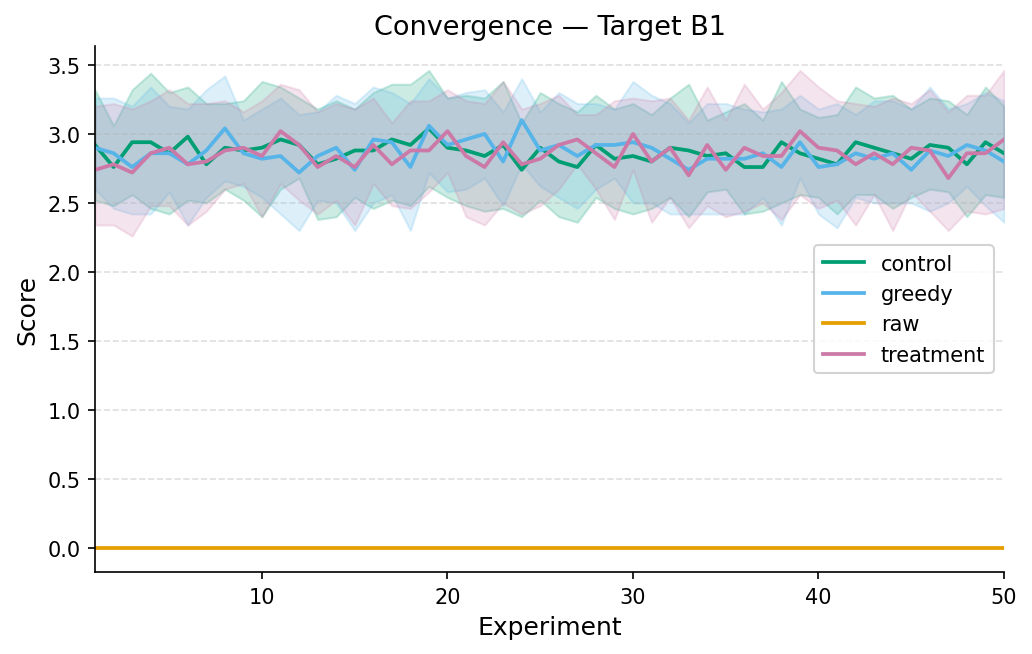
\includegraphics[width=0.195\textwidth]{figures/convergence/convergence_B1.png}\hfill
  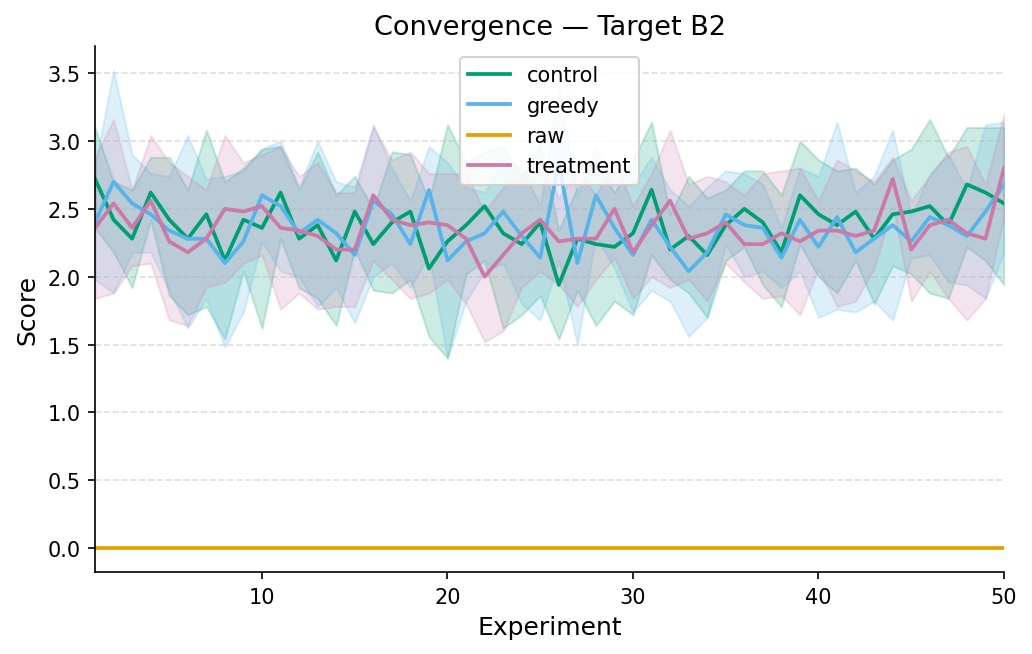
\includegraphics[width=0.195\textwidth]{figures/convergence/convergence_B2.png}\hfill
  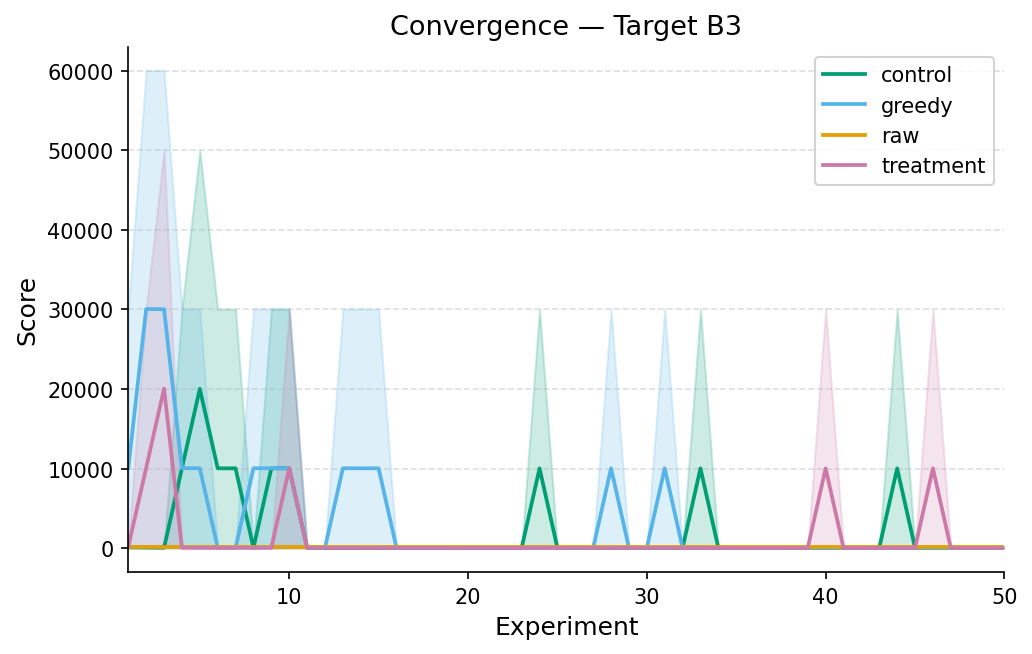
\includegraphics[width=0.195\textwidth]{figures/convergence/convergence_B3.png}\hfill
  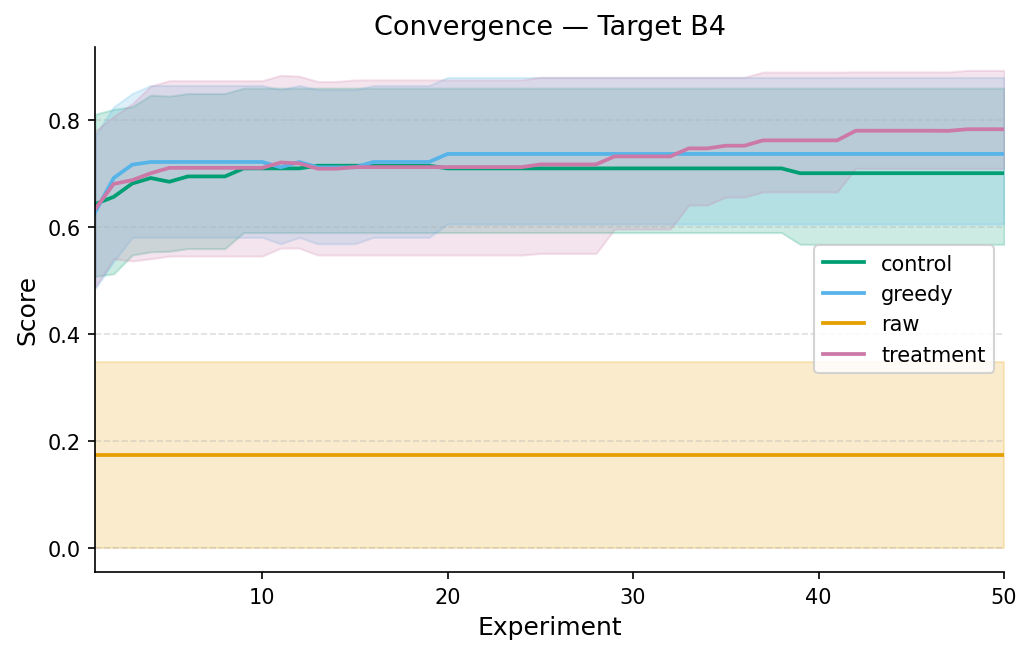
\includegraphics[width=0.195\textwidth]{figures/convergence/convergence_B4.png}\hfill
  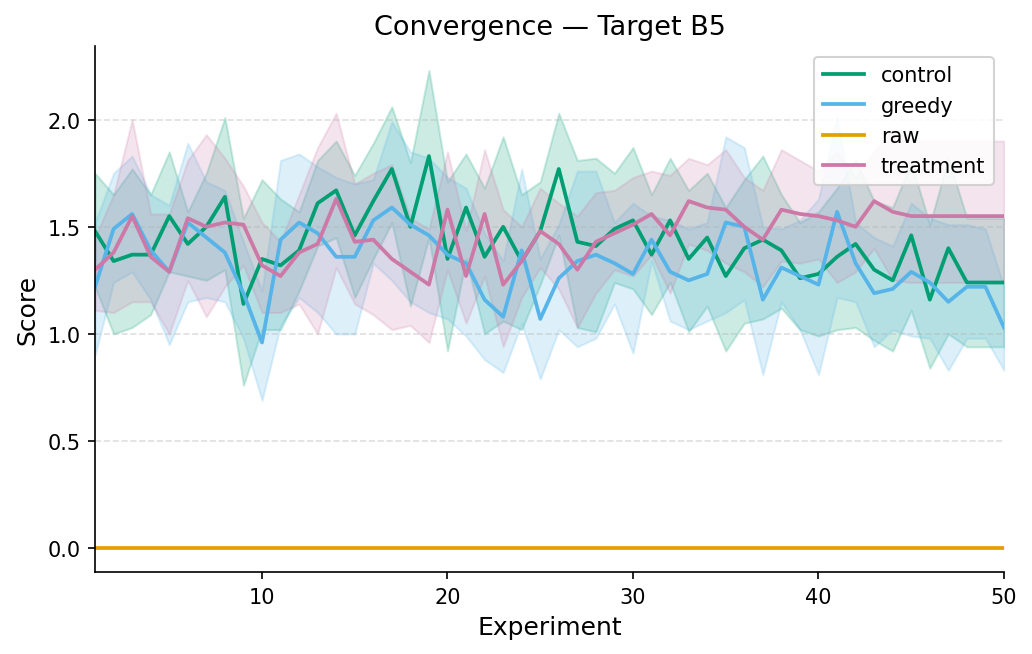
\includegraphics[width=0.195\textwidth]{figures/convergence/convergence_B5.png}
  \Description{Five line plots, one per benchmark target B1 through B5, showing mean final score versus experiment index with one line per configuration (greedy, control, treatment) and shaded standard deviation across the five paired seeds.}
  \caption{Per-experiment convergence trajectories on B1--B5 across the five paired seeds. Each panel plots mean final-score vs.\ experiment index for greedy, control, and treatment; shaded bands show the seed-level standard deviation. Generated by \texttt{benchmarks/analysis/convergence.py} from \texttt{benchmarks/raw\_results\_seeds1-5/}.}
  \label{fig:convergence-strip}
\end{figure*}
The treatment configuration produces a directional improvement over the control configuration on all five targets: $\deltaTCBone\%$ on B1, $\deltaTCBtwo\%$ on B2, $\deltaTCBthreeArith\%$ on B3 (B3 minimizes), $\deltaTCBfour\%$ on B4, and $\deltaTCBfive\%$ on B5.
The treatment configuration also produces a directional improvement over the greedy configuration on all five targets, ranging from $+4.5\%$ on B2 to $+87.8\%$ on B5.
The largest configuration gap is between any optimization configuration and the raw baseline, where the engine reliably moves the artifact away from a starting point that scores zero (B1, B2, B5) or near-zero (B4) on the evaluation rubric.
B3 is noisier: its raw mean is much worse than treatment, while its raw median is zero in the generated summary because several raw executions hit the parser's best-case floor while others are extreme slow outliers.\footnote{The B3 raw-mean (185.68\,ms) and raw-median (0\,ms) divergence reflects this bimodal distribution: roughly half of the seeds produce trivially-fast outputs that the parser clamps at the floor, while the rest are slow outliers that dominate the mean. Treatment mutations bring all five seeds into a compact mid-range distribution, eliminating both modes.}

\begin{table}[t]
  \centering
  \caption{Mean final score per target $\times$ configuration across $n = 5$ paired seeds, with relative change of treatment over control. Direction column indicates whether the metric is maximized ($\uparrow$) or minimized ($\downarrow$).}
  \label{tab:e2e-final-scores}
  \small
  \begin{tabular}{@{}llrrrrr@{}}
    \toprule
    Target & Dir. & raw & greedy & control & treatment & $\Delta_{T/C}$ \\
    \midrule
    B1 & $\uparrow$  & 0.00   & 2.80   & 2.86  & 2.96  & $+3.5\%$  \\
    B2 & $\uparrow$  & 0.00   & 2.68   & 2.54  & 2.80  & $+10.2\%$ \\
    B3 & $\downarrow$ & 185.68 & 103.68 & 72.81 & 40.38 & $-44.5\%$ \\
    B4 & $\uparrow$  & 0.17   & 0.74   & 0.70  & 0.78  & $+11.7\%$ \\
    B5 & $\uparrow$  & 0.00   & 0.82   & 1.30  & 1.54  & $+18.5\%$ \\
    \bottomrule
  \end{tabular}
\end{table}

\subsubsection{Statistical Significance}
\label{sec:end-to-end-significance}

The directional pattern above is consistent across targets, but the framework's own statistical-acceptance discipline is the right standard against which to test it.
\Cref{tab:e2e-stats} reports the Wilcoxon signed-rank $p$-value for each pairwise comparison together with the Holm--Bonferroni-corrected $p$-value across the five targets and Cohen's $d$ with bootstrap 95\% confidence intervals.
The corrected significance threshold is $\alpha = 0.05$.

\begin{table}[t]
  \centering
  \caption{Pairwise comparisons of final score across configurations at $n = 5$ paired seeds per target. $p_{\text{raw}}$ is the Wilcoxon signed-rank $p$-value; $p_{\text{corr}}$ is the Holm--Bonferroni-corrected $p$-value across the five-target family; $d$ is Cohen's $d$ with bootstrap 95\% CI (10{,}000 resamples). Significance is reported at $\alpha = 0.05$ on $p_{\text{corr}}$.}
  \label{tab:e2e-stats}
  \scriptsize
  \begin{tabular}{@{}llrrrl@{}}
    \toprule
    Target & Comparison & $p_{\text{raw}}$ & $p_{\text{corr}}$ & $d$ & 95\% CI \\
    \midrule
    B1 & control vs.\ treatment & 0.625 & 1.000 & 0.18  & $[-1.25, 2.26]$ \\
    B2 & control vs.\ treatment & 0.250 & 1.000 & 0.41  & $[-1.25, 1.96]$ \\
    B3 & control vs.\ treatment & 0.625 & 1.000 & $-0.53$ & $[-2.28, 0.82]$ \\
    B4 & control vs.\ treatment & 0.250 & 1.000 & 0.51  & $[-0.75, 2.25]$ \\
    B5 & control vs.\ treatment & 0.625 & 1.000 & 0.36  & $[-1.25, 1.72]$ \\
    \midrule
    B1 & greedy vs.\ treatment  & 0.250 & 0.750 & 0.26  & $[-1.09, 2.13]$ \\
    B2 & greedy vs.\ treatment  & 0.750 & 1.000 & 0.21  & $[-1.24, 1.76]$ \\
    B3 & greedy vs.\ treatment  & 0.062 & 0.312 & $-1.09$ & $[-3.86, 0.03]$ \\
    B4 & greedy vs.\ treatment  & 0.625 & 1.000 & 0.30  & $[-1.09, 1.74]$ \\
    B5 & greedy vs.\ treatment  & 0.062 & 0.312 & 1.35  & $[\phantom{-}0.46, 3.41]$ \\
    \midrule
    B1 & raw vs.\ treatment     & 0.062 & 0.312 & 6.59  & $[\phantom{-}5.40, 24.96]$ \\
    B2 & raw vs.\ treatment     & 0.062 & 0.312 & 8.00  & $[\phantom{-}6.18, 21.98]$ \\
    B3 & raw vs.\ treatment     & 0.812 & 0.812 & $-0.79$ & $[-2.35, 1.65]$ \\
    B4 & raw vs.\ treatment     & 0.062 & 0.312 & 3.20  & $[\phantom{-}2.64, 13.33]$ \\
    B5 & raw vs.\ treatment     & 0.062 & 0.312 & 3.06  & $[\phantom{-}2.12, \phantom{0}9.30]$ \\
    \bottomrule
  \end{tabular}
\end{table}

\paragraph{What the corrected $p$-values say.}
No comparison reaches significance after Holm--Bonferroni correction at $n = 5$ paired seeds across the five-target family.
The two strongest non-raw signals are the treatment-versus-greedy comparisons on B3 ($d = -1.09$, 95\% CI nearly excludes zero, $p_{\text{corr}} = 0.312$) and on B5 ($d = 1.35$, 95\% CI excludes zero, $p_{\text{corr}} = 0.312$).
Their uncorrected $p$-values are both $0.062$, the smallest the Wilcoxon test can produce at $n = 5$ paired observations: even a perfect 5/5 directional sweep does not clear the corrected threshold under a five-target correction.
The treatment-versus-control effect sizes are small to large across targets ($d \in [-0.53, 0.51]$ on the original sign convention; B3's negative $d$ corresponds to a $44.5\%$ improvement under minimization), and the Wilcoxon test does not reject the null at the corrected threshold.

\paragraph{Why this is the right standard.}
The non-significance of treatment-versus-control after correction is the framework's statistical acceptance discipline applied to itself.
A point-score comparison of the same data would report ``treatment beats control on 5/5 targets'' as a victory; the same comparison run with the engine's own machinery (paired Wilcoxon, multiplicity correction across the five-target family) declines to make that claim at $n = 5$ paired seeds.
The Wilcoxon test's minimum attainable $p$-value at $n = 5$ is $1/2^5 = 0.03125$ for a one-sided test and $0.0625$ for a two-sided test, so even a perfect 5/0 sign sweep within a target sits just above the per-comparison threshold and well above the corrected one.
This is the same conservatism that \cref{sec:gate-false-positives} validated on a synthetic null: the multiplicity correction does not produce false-positive headlines, and at this seed count it requires effect sizes well into Cohen's-large territory or perfect directional consistency in conjunction with a less aggressive correction to reject the null.
The directional pattern across targets and the two strongest B3/B5 greedy-versus-treatment comparisons identify where a higher-powered replication would be most informative.
We discuss this and the implications for interpretation in \cref{sec:threats}.

\subsubsection{Cost Telemetry}
\label{sec:end-to-end-cost}

\Cref{tab:e2e-cost} reports the mean USD cost per seed for the three optimization configurations on each target.
The raw configuration is omitted because it incurs no LLM cost beyond initial-artifact generation.
Treatment cost is within the same order as control cost under the archived model-routing setup: it is higher on B1 and B3, lower on B2, B4, and B5.
Because the archived records were generated under mixed model routing and one draft per experiment (\cref{tab:result-provenance}), these numbers should be interpreted as cost telemetry for this run, not as evidence that specific enhancement mechanisms are cost-neutral.

\begin{table}[t]
  \centering
  \caption{Mean USD cost per seed across configurations, by target (\texttt{total\_cost\_usd} aggregated over the experiment budget, $n = 5$ seeds). These are archived telemetry values under the mixed model-routing setup in \cref{tab:result-provenance}; raw is excluded because its recorded optimization-loop cost is zero.}
  \label{tab:e2e-cost}
  \small
  \begin{tabular}{@{}lrrr@{}}
    \toprule
    Target & greedy (\$) & control (\$) & treatment (\$) \\
    \midrule
    B1 & 2.59 & 2.19 & 2.72 \\
    B2 & 2.64 & 3.12 & 2.86 \\
    B3 & 2.28 & 3.12 & 3.46 \\
    B4 & 1.20 & 1.57 & 1.50 \\
    B5 & 7.56 & 7.53 & 6.71 \\
    \bottomrule
  \end{tabular}
\end{table}

The combined view of \cref{tab:e2e-final-scores,tab:e2e-cost} is that treatment has the strongest directional final scores while remaining within the same cost range as control in this archived run.
The table does not identify which internal feature accounts for cost movement, because the run does not isolate multi-draft, two-phase, dual-agent, or model-routing effects independently.

\subsubsection{Illustrative Trajectory: B4 Code Quality}
\label{sec:end-to-end-illustrative}

To make the abstract numbers concrete, consider one trajectory of the treatment configuration on B4.
The seed artifact is a single-file CRUD endpoint of $\sim 60$ lines: validation absent or stringly-typed, exception handling reduced to a bare \texttt{except} that returns a generic \texttt{500}, timestamps stored as \texttt{str(datetime.now())}, no input bounds, no audit logging.
Under the deterministic composite scorer (correctness via a hidden test suite, plus lint compliance scaled by violation count), this artifact scores $\bar{x}_{\text{raw}} = 0.174$ across the five seeds.
On the first accepted treatment mutation of seed 1, the agent rewrote the file end-to-end: typed pydantic-style request models, explicit email-format and age-range validation with \texttt{422} responses, structured exception handling with distinct status codes for validation versus internal errors, and ISO-formatted timestamps via \texttt{datetime.isoformat}.
The composite score moved from $0.435$ at the seed's pre-experiment baseline to $0.9$ after the mutation, a single-step jump that the framework's statistical-acceptance layer then preserved as the reference baseline for subsequent experiments.
This pattern (a large early jump from the raw artifact, followed by smaller incremental refinements that the multiplicity-corrected acceptance layer admits selectively) is consistent with the per-target descriptive statistics in \cref{tab:e2e-final-scores}.
The full per-experiment trajectories for every seed and configuration are shipped as JSONL in \texttt{benchmarks/raw\_results\_seeds1-5/}.

\subsubsection{Configuration-Step Differences}
\label{sec:end-to-end-ablation}

The four configurations of \cref{tab:e2e-configs} can be read as descriptive steps from less machinery to more machinery, but they do not isolate the independent contribution of each enhancement.
\Cref{tab:e2e-marginal} therefore reports configuration-step differences on the final-score metric, not marginal causal effects.

\begin{table}[t]
  \centering
  \caption{Descriptive configuration-step differences on the final-score metric, per target ($n = 5$ paired seeds). Each cell is the relative change in mean final score between adjacent named configurations. Sign is normalized so that positive numbers represent improvement (B3 minimizes, so its sign is flipped). Cells marked ``--'' are undefined because the raw baseline mean is zero. The rightmost column is the cumulative difference of treatment over raw, where well-defined.}
  \label{tab:e2e-marginal}
  \scriptsize
  \begin{tabular}{@{}lrrrr@{}}
    \toprule
    Target & raw $\to$ greedy & greedy $\to$ control & control $\to$ treatment & raw $\to$ treatment \\
            & (greedy search)  & (+hybrid default) & (+treatment bundle)   & (cumulative)        \\
    \midrule
    B1 & --      & $+2.1\%$  & $+3.5\%$  & -- \\
    B2 & --      & $-5.2\%$  & $+10.2\%$ & -- \\
    B3 & $+44.2\%$ & $+29.8\%$ & $+44.5\%$ & $+78.2\%$ \\
    B4 & $+323\%$  & $-5.0\%$  & $+11.7\%$ & $+350\%$ \\
    B5 & --      & $+58.5\%$ & $+18.5\%$ & -- \\
    \bottomrule
  \end{tabular}
\end{table}

The raw $\to$ greedy column is reported only for targets where the raw mean is non-zero, since percentage change from a zero baseline is undefined.
On the four targets where the greedy $\to$ control transition is well-defined alongside the rest of the chain, control improves over greedy on three of them; the regressions on B2 and B4 are small in absolute terms and within the seed-level standard deviation, consistent with sampling noise at $n = 5$.
The control $\to$ treatment transition is positive on all five targets, ranging from $\deltaTCBone\%$ to $\deltaTCBthree\%$.
This table is useful for locating where the named configurations differ most, but it does not identify which member of the treatment bundle caused the difference.

% ==================================================================
\subsection{Synthesis}
\label{sec:empirical-scope}

The mechanism gates and the end-to-end comparison together establish the strongest claim the data support: the validated subsystems behave as specified in isolation, and the archived treatment configuration improves over greedy hill-climbing and over control on every target in the shipped suite.
The framework's own statistical discipline declines to call this gap significant after multiplicity correction at $n = 5$ paired seeds across the five-target family.
We treat this conservatism as a feature: the same machinery that produced the 86\% false-positive reduction in \cref{sec:gate-false-positives} imposes a stricter standard on systemic claims here, and the strongest B3 and B5 greedy-versus-treatment effects ($d = -1.09$ and $d = 1.35$, $p_{\text{corr}} = 0.312$) identify the comparisons a future higher-powered replication should prioritize.
The threats-to-validity discussion in \cref{sec:threats} elaborates on what the seed count can and cannot resolve, and on the construct-validity considerations specific to LLM-judge evaluation.

% !TEX root = ../main.tex
\section{Discussion}
\label{sec:discussion}

\subsection{Limitations}
\label{sec:limitations}

\paragraph{Single-agent mutation.}
Each experiment cycle invokes exactly one mutation agent that edits the artifact in isolation, so mutations that require coordinated changes across interacting files cannot be generated atomically: an edit to a function signature and its call sites must either be proposed as a single multi-file patch by one agent or deferred across multiple experiment cycles.
The current architecture does not support multi-agent coordination with conflict resolution or merge semantics, so optimization targets whose improvements fundamentally require parallel specialization (one agent refactoring structure while another refines documentation) fall outside the framework's reach.

\paragraph{Text artifacts only.}
The engine operates on file-based text artifacts versioned in git.
Binary files (images, compiled assets, database schemas), structured data stores, and deployed services are outside the mutation scope.
Optimization targets requiring deployment to external systems (email campaigns, ad platforms) are supported only as read-only proposal generation with approval gates; this pathway is implemented but not evaluated here, and it is not integrated with external deployment systems.

\paragraph{LLM-as-judge evaluation quality.}
Stochastic evaluation relies on an LLM judge scoring against binary criteria.
The quality of optimization is bounded by the quality of the judge: a judge that rewards superficial keyword matching will drive the optimizer toward keyword-stuffed artifacts.
Position debiasing (\cref{sec:eval-pipeline}) and held-out validation mitigate systematic judge bias, but they do not eliminate it.
Practitioners must invest in evaluation design (clear, unambiguous criteria with concrete acceptance thresholds) to obtain meaningful optimization trajectories.

\paragraph{Cost.}
A full optimization run of 50 experiments incurs substantial LLM API cost, with the exact figure depending on the evaluation mode, the number of stochastic samples per experiment, and the selected models for the mutation, diagnosis, and judgment roles.
Two-phase mutation and multi-draft generation can increase per-experiment cost relative to single-phase greedy mutation because of the additional LLM calls for diagnosis and draft generation.
For cost-sensitive applications, the engine supports cheaper diagnosis models (e.g., a smaller model for diagnosis and a larger one for mutation) and adaptive sample sizing that reduces evaluation cost for clear winners and losers.

\paragraph{Cold start.}
The knowledge system provides no benefit during the first several experiments, when the experiment history is empty.
The TF-IDF retrieval index requires a minimum corpus size before similarity queries become discriminative, and the engine's cold-start protocol injects only raw experiment records until a configurable activation threshold is reached.

\subsection{Threats to Validity}
\label{sec:threats}

\paragraph{Internal validity.}
LLM outputs are nondeterministic: the same prompt produces different mutations across runs.
We control for this by pairing runs by random seed across configurations and using nonparametric statistical tests that do not assume distributional form.
API pricing variability, model availability changes, backend switching, rate limits, and transient retry behavior introduce noise into cost measurements.
The archived end-to-end records include mixed model routing (\cref{tab:result-provenance}), so the cost tables should be interpreted as telemetry for that result bundle rather than as provider-independent cost estimates.
The analysis mitigates billing opacity by reading recorded per-experiment cost fields instead of relying on billing-console totals.

\paragraph{Empirical scope and statistical power.}
The end-to-end comparison in \cref{sec:end-to-end} runs at $n = 5$ paired seeds per target across five targets.
At this seed count the Wilcoxon signed-rank test has a two-sided $p$-value floor of $0.0625$, so no comparison can reach the conventional $\alpha = 0.05$ threshold per-target without ties or unusual sign patterns, and after Holm--Bonferroni correction across five targets the bar rises further still.
The directional pattern across targets (treatment beats control on 5/5 targets, treatment beats greedy on 5/5 targets) and the Cohen's-large effect sizes on the two strongest greedy-versus-treatment comparisons (B3, $d = -1.09$; B5, $d = 1.35$) indicate that seed count is one binding constraint on whether systemic claims clear the corrected threshold.
A higher-powered replication (larger $n$ per target, or a study restricted to one or two targets that does not pay the five-target multiplicity tax) would test whether the directional advantage of the treatment configuration translates into a statistically defensible claim.
We have intentionally not run such a replication at this stage because the seed-counted result with its honest non-significance is more informative than a cherry-picked single-target study would be: it illustrates exactly the conservatism the framework's statistical-acceptance layer is designed to enforce.
The domain-agnostic design claim in \cref{sec:introduction} continues to rest primarily on the architecture of the artifact--evaluation--agent triplet (\cref{sec:triplet}); the suite spans prompts, code, and documentation, but five targets cannot establish that the framework composes into improvements across the broader space of text-artifact optimization problems.

\paragraph{External validity.}
The five benchmark targets that ship with the framework are themselves a simplification of real-world optimization problems.
Production artifacts are larger, have more complex dependency structures, and operate under constraints (backward compatibility, style guides, regulatory requirements) that the benchmark targets do not capture.
The benchmark suite is intended as a reproducible reference workload for comparing configurations under controlled conditions, not as a representative sample of the distribution of problems a practitioner would encounter in practice.
The suite is useful for controlled comparison and failure analysis, but it does not establish that relative ordering of configurations will transfer unchanged to production-scale artifacts.

\paragraph{Construct validity.}
Stochastic evaluation quality depends on the specificity and completeness of the scoring criteria.
Vague criteria (e.g., ``is the output high quality?'') produce noisy scores that obscure real improvements.
The benchmark targets ship with criteria that are phrased as concrete yes/no questions with explicit acceptance conditions, and the position-bias cancellation and Bradley--Terry scoring described in \cref{sec:eval-pipeline} further reduce judge-level artefacts.
This investment in criterion design is itself a limitation: in practice, users may not invest equivalent effort, leading to lower optimization effectiveness than the benchmark design suggests.

\paragraph{Proxy gaming and rubric-facing optimization.}
The architectural separation in \cref{sec:triplet} (immutable eval definitions, an agent that never sees the eval command, scope enforcement that blocks edits to scoring code) prevents the agent from modifying the evaluation function itself.
It does not prevent the agent from optimizing the evaluation function as it is written.
On stochastic-eval targets, an agent can learn to produce artifacts that score well on the rubric criteria as phrased even when the produced artifact does not match the rubric's intent: rubric-facing language that satisfies a binary keyword check, formatting choices that satisfy a structural criterion without addressing the underlying quality the criterion is meant to proxy, or coverage of all listed cases without depth on any of them.
On deterministic-eval targets, an agent can overfit to the test fixtures: passing the specific inputs the harness exercises while degrading on inputs the harness does not exercise.
The framework's defense against these failure modes is external to the optimization loop---held-out divergence detection (\cref{sec:eval-pipeline}) flags artifacts whose held-out and primary-set scores diverge---but the user remains responsible for designing rubrics and harnesses where the proxy is closely aligned with the intent.
Where alignment is weak, the framework will optimize the proxy, not the intent.

\subsection{Future Work}
\label{sec:future-work}

\paragraph{Higher-powered empirical replication.}
The seed-counted end-to-end study in \cref{sec:end-to-end} establishes a consistent directional advantage of the treatment configuration over both control and greedy across the suite, but does not clear the multiplicity-corrected significance threshold at $n = 5$.
The two strongest greedy-versus-treatment comparisons (B3, B5) sit at the Wilcoxon two-sided $p$-value floor for $n = 5$, indicating that statistical power is one unresolved constraint on the systemic claim.
A replication at higher seed counts on a smaller subset of targets would resolve whether the directional advantage translates into a statistically defensible claim.

\paragraph{Multi-artifact optimization.}
Extending the mutation scope to coordinated changes across multiple files (e.g., modifying a function signature and all its call sites simultaneously) would enable structural refactoring that single-file mutations cannot achieve.
This requires dependency-aware scoping and atomic multi-file commits with rollback semantics, both of which the git environment backend supports in principle.

\paragraph{Typed evaluator protocol.}
The current evaluation interface is command-based: the engine invokes a shell command and parses its stdout.
A typed Python callable protocol (already prototyped in the codebase) would enable programmatic evaluation with structured return types, eliminating parsing fragility and supporting evaluation functions that require in-process state (database connections, loaded ML models).

\paragraph{MAP-Elites integration.}
The quality-diversity archive (\cref{sec:enhancements}) maintains a grid of behaviorally diverse solutions but is not yet integrated into the search loop as a solution source.
Full MAP-Elites integration would allow the engine to optimize for diversity and quality simultaneously, producing a portfolio of distinct high-scoring artifacts rather than a single best solution.

\paragraph{Continuous optimization.}
A daemon mode that monitors artifact changes and triggers optimization runs on detected regressions would enable always-on quality maintenance.
The scheduler and daemon management components are implemented; the remaining work is policy design for when to trigger optimization (commit hooks, schedule, metric drift detection) and how to surface results without disrupting the developer workflow.

\paragraph{IDE integration.}
Embedding the optimization loop into editor extensions (VS Code, JetBrains) would reduce the barrier to adoption by allowing developers to trigger optimization on selected files without leaving their editor.
The engine's file-based architecture (JSONL logs, file-based SSE dashboard) is compatible with extension integration, but the UX design (progress visualization, result acceptance, inline diff preview) remains open.

% !TEX root = ../main.tex
\section{Conclusion}
\label{sec:conclusion}

We presented \textsc{anneal}, an interface-level domain-agnostic framework that brings statistical decision theory to the accept/reject boundary of iterative LLM-guided artifact optimization.
The system operates on the minimal abstraction of an (Artifact, Eval, Agent) triplet: given any measurable artifact and an evaluation function, an LLM agent generates informed mutations, the engine evaluates them under statistical rigor, and a search strategy decides whether to accept or revert each change.
Every experiment is git-committed, scope-enforced, and logged.

The framework's three technical contributions (statistical acceptance under stochastic evaluation, adaptive metaheuristic search, and structured episodic knowledge retrieval) are each evaluated as an independent mechanism in \cref{sec:results}.
Holm--Bonferroni correction reduces false-positive acceptance by \fpReductionPct\% under a synthetic null distribution (\cref{sec:gate-false-positives}), adaptive simulated annealing yields a directional \saImprovementPct\% improvement over fixed cooling on the 3D Rastrigin function while narrowly missing the precommitted 15\% gate (\cref{sec:gate-sa}), and TF-IDF retrieval achieves $\retrievalRatio\times$ the precision of Jaccard similarity on a controlled corpus (\cref{sec:gate-retrieval}).
These mechanism-level results are supported by two architectural contributions (git-native isolation with scope enforcement, and a domain-agnostic artifact--evaluation interface) that realize the framework as an integrated, reproducible research artifact.

The exploratory end-to-end study of \cref{sec:end-to-end} compares four configurations (raw, greedy, control, treatment) on the five-target benchmark suite at $n = 5$ paired seeds.
The archived treatment configuration produces a directional improvement on final-score over control on every target, ranging from $\deltaTCBone\%$ to $\deltaTCBthree\%$, with mean cost in the same range under the recorded model-routing setup.
After Holm--Bonferroni correction across the five-target family, no treatment-versus-control or treatment-versus-greedy comparison reaches significance at the seed count run; the strongest greedy-versus-treatment effects (B3 and B5) sit at the Wilcoxon two-sided floor of $p = 0.0625$ before correction.
The benchmark targets, raw per-seed result files, and analysis pipeline ship as part of the open-source distribution so that readers can inspect the archived evidence and extend the suite.
The highest-priority extensions are higher-powered replications resolving the open near-significant comparisons and multi-artifact coordinated mutations that lift the current single-file scope (\cref{sec:future-work}).

\textsc{anneal} is available under the Apache-2.0 license at \url{https://github.com/Mathews-Tom/anneal} and as the \texttt{anneal-cli} package on PyPI.


%%
%% Bibliography
%%
\bibliographystyle{plainnat}
\bibliography{references}

\end{document}
